\documentclass[11pt]{beamer}
\setbeamertemplate{navigation symbols}{}

\usepackage[utf8]{inputenc}
\usepackage[T1]{fontenc}
\usepackage{libertine}

\usepackage{pgfplots} 		% For plotting data. Also loads TikZ.
%\usepackage{pgfplotstable}
\pgfplotsset{compat=1.11}
\usetikzlibrary{intersections}
\usetikzlibrary{external}						% for building images only when it's needed
\tikzexternalize[prefix=./plots/]		% activate the library and place the images in the "images/tikz/" subfolder
%\tikzset{external/force remake} 		% force remake of all images

\title{Pgfplots and TikZ data example}
\author{Matteo Sostero}

\begin{document}

\begin{frame}{Simple function with \texttt{TikZ}}
\centering
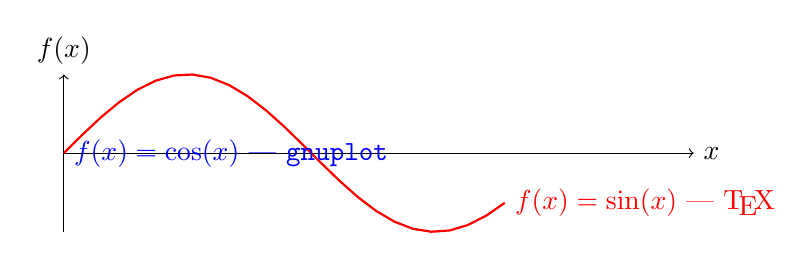
\begin{tikzpicture}[domain=0:5.6]
\draw[->] (0,0) -- (8,0) node[right] {$x$};
\draw[->] (0,-1) -- (0,1) node[above] {$f(x)$};
\draw[color=red,thick] plot (\x,{sin(\x r)}) node[right] {$f(x) =\sin (x)$ — \TeX};														% using the TeX engine
\draw[color=blue,thick] plot[id=cosx] function{cos(x)} node[right] {$f(x) =\cos (x)$ — \texttt{gnuplot}} ; 	% using GNUPLOT 
\end{tikzpicture}
\end{frame}


\begin{frame}{Function plotting with \texttt{PGF}}
\centering
\begin{tikzpicture}
\begin{axis}[
	width=10cm, height=8cm,
	% some fine-tuning for the display:
	samples=1000,
	restrict y to domain=-10:10,
	xmin=-5, xmax=5,
	xtick={-4.7124,-1.5708,...,10},
	xticklabels={$-\frac32 \pi$,$-\frac\pi2$,$\frac\pi2$,$\frac32 \pi$},
	axis x line=center,
	axis y line=center,
	legend cell align=left]
\addplot[blue,domain=-1.5*pi:1.5*pi] {tan(deg((x))};
\addplot[red] gnuplot[id=tangens,domain=-1.5*pi:1.5*pi] {tan(x-pi/2)};
\legend{$\tan(x)$ (pgf), $\tan\left(x-\frac\pi 2\right)$ (gnuplot)}
\end{axis}
\end{tikzpicture}
\end{frame}


\begin{frame}{Loading data from\texttt{.dat} file}
\centering
\begin{tikzpicture}
\begin{axis}[
	title={Plot of $\sin\left(\frac1 x\right)$},
	width=10cm, height=8cm,xtick={0,0.1},ytick={-1,0,1}]
\addplot[blue,thin] table {./data.dat};
\end{axis}
\end{tikzpicture}
\end{frame}

\begin{frame}{Level curves using \texttt{gnuplot}}
\centering
\begin{tikzpicture} 
\begin{axis}[
	title={Level curves of $z(x,y)=xy$},
	view={0}{90}] 
\addplot3[contour gnuplot] {x*y}; 
\end{axis} 
\end{tikzpicture}
\end{frame}


\begin{frame}{Surface Plot}
\centering
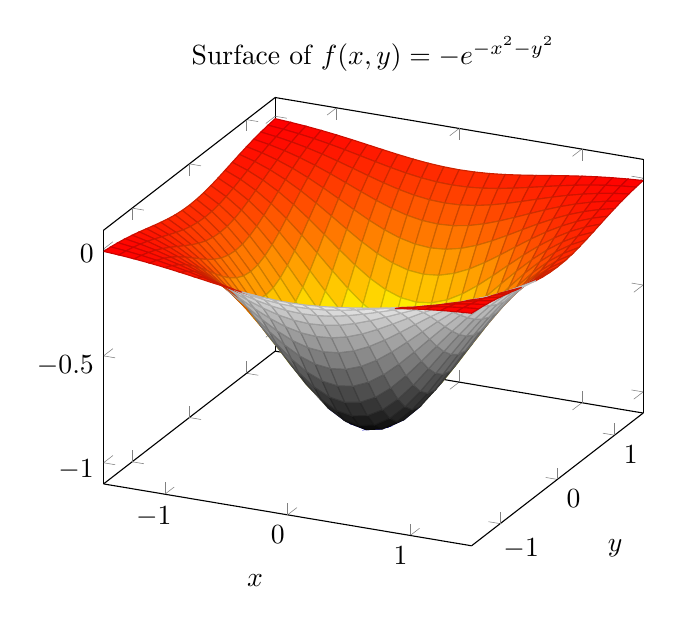
\begin{tikzpicture} 
\begin{axis}[
	title={Surface of $f(x,y)=-e^{-x^2-y^2}$},
	xlabel=$x$,ylabel=$y$,
	mesh/interior colormap name=hot, 
	colormap/blackwhite]
\addplot3[domain=-1.5:1.5,surf] {-exp(-x^2-y^2)}; 
\end{axis}
\end{tikzpicture}
\end{frame}


\begin{frame}{Curve-bending}
\centering
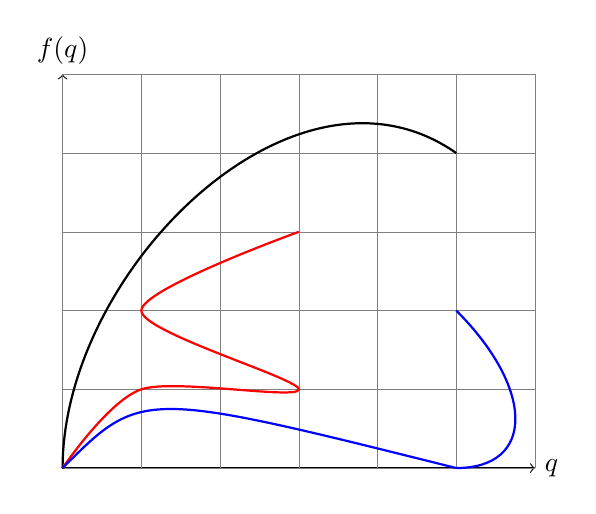
\begin{tikzpicture}
\draw[<->] (6,0) node[right]{$q$} -- (0,0) --(0,5) node[above]{$f(q)$};
\draw[help lines] grid (6,5);
\draw[thick] (0,0) to [out=90,in=145] (5,4);
\draw[thick,red] plot [smooth] coordinates {(0,0) (1,1) (3,1) (1,2) (3,3)};
\draw[thick,blue] (0,0) .. controls (1,1) .. (5,0)  (5,0) .. controls (6,0) and (6,1) .. (5,2);
\end{tikzpicture}
\end{frame}
\end{document}